\documentclass[conference]{IEEEtran}
\IEEEoverridecommandlockouts
% The preceding line is only needed to identify funding in the first footnote. If that is unneeded, please comment it out.
%Template version as of 6/27/2024

\usepackage{cite}
\usepackage{amsmath,amssymb,amsfonts}
\usepackage{algorithmic}
\usepackage{graphicx}
\usepackage{textcomp}
\usepackage{xcolor}
\usepackage{verbatim}
\newcommand{\blue}[1]{\textcolor{blue}{#1}}
\newcommand{\red}[1]{\textcolor{red}{#1}}
\usepackage{comment}
\usepackage[table]{xcolor}
\usepackage{booktabs}
\usepackage{multirow}
\def\BibTeX{{\rm B\kern-.05em{\sc i\kern-.025em b}\kern-.08em
    T\kern-.1667em\lower.7ex\hbox{E}\kern-.125emX}}
\begin{document}

\title{Distributional Baselines for Conversational Prosody and Rhythm\\
\thanks{Identify applicable funding agency here. If none, delete this.}
}

\author{
\IEEEauthorblockN{Author Names Omitted for Review}
\IEEEauthorblockA{
Affiliations omitted for review\\
Email omitted for review}
}

\begin{comment}
\author{\IEEEauthorblockN{1\textsuperscript{st} Given Name Surname}
\IEEEauthorblockA{\textit{dept. name of organization (of Aff.)} \\
\textit{name of organization (of Aff.)}\\
City, Country \\
email address or ORCID}
\and
\IEEEauthorblockN{2\textsuperscript{nd} Given Name Surname}
\IEEEauthorblockA{\textit{dept. name of organization (of Aff.)} \\
\textit{name of organization (of Aff.)}\\
City, Country \\
email address or ORCID}
\and
\IEEEauthorblockN{3\textsuperscript{rd} Given Name Surname}
\IEEEauthorblockA{\textit{dept. name of organization (of Aff.)} \\
\textit{name of organization (of Aff.)}\\
City, Country \\
email address or ORCID}
\and
\IEEEauthorblockN{4\textsuperscript{th} Given Name Surname}
\IEEEauthorblockA{\textit{dept. name of organization (of Aff.)} \\
\textit{name of organization (of Aff.)}\\
City, Country \\
email address or ORCID}
\and
\IEEEauthorblockN{5\textsuperscript{th} Given Name Surname}
\IEEEauthorblockA{\textit{dept. name of organization (of Aff.)} \\
\textit{name of organization (of Aff.)}\\
City, Country \\
email address or ORCID}
\and
\IEEEauthorblockN{6\textsuperscript{th} Given Name Surname}
\IEEEauthorblockA{\textit{dept. name of organization (of Aff.)} \\
\textit{name of organization (of Aff.)}\\
City, Country \\
email address or ORCID}
}
\end{comment}

\maketitle

\begin{abstract}
Speech-to-speech (S2S) AI agents are advancing rapidly, yet evaluation remains dominated by text-centric measures, task success, or subjective ratings that do not directly capture conversational naturalness. 
We analyze 4000+ hours of dyadic English conversation from the Seamless Interaction dataset to derive speech-native reference distributions. 
We compute prosodic (Mean, Range, \& Standard Deviation of F0) and temporal (Speech \& Articulation Rate, Pause Ratio) operating regimes and quantify how they shift with speaker (gender and age) and interaction (arousal and dominance) factors.
These empirically grounded regimes provide calibrated targets for speech-native, multi-cue evaluation of interaction quality, intending to support future approaches that combine multiple cues to detect and characterize unnatural speech in S2S dialogue model outputs.
\end{abstract}

\begin{IEEEkeywords}
Distributional Baselines, Conversational Speech, Naturalness Evaluation, Metric Regimes
\end{IEEEkeywords}

\section{Introduction}

Spoken conversation is a highly coordinated form of communication, where interlocutors manage turn-taking while continuously adapting prosody and timing to the unfolding interaction \cite{riest_anticipation_2015, levinson_turn-taking_2016}. 
Despite this complexity, transitions are typically smooth and supported by systematic cues, including prosodic and syntactic structure \cite{koiso_analysis_1998}.
Speech technology has progressed toward S2S AI agents capable of producing fluent spoken responses. 
Evaluation, however, is still dominated by text-based measures, task success, or subjective ratings, which do not directly quantify speech-native interactional behavior. 
Systems trained primarily on read speech often fail to reproduce properties characteristic of spontaneous dialogue \cite{omahony_combining_2022}.

Conversational speech differs from read speech across multiple dimensions, including prosodic range and stress realization \cite{howell1991comparison, hazan2010does}. 
Temporal organization varies with context and listener demands, shaping speaking rate and rhythmic structure \cite{tauroza_speech_1990, ward_automatic_2004, dowding_user_2024, xie_speaking_2024}. 
These patterns align with accounts of dialogue as adaptive coordination, where speakers modify behavior to meet various contextual demands \cite{fusaroli_dialog_2014, wynn_conversational_2024}.

Prosodic variation, particularly fundamental frequency ($F_0$), encodes communicative intent, emotion, and discourse structure, and interacts with prominence and stress cues \cite{banziger_role_2005, pell_emotional_2011, xu_speech_2005, sluijter_acoustic_1996, sluijter_spectral_1996}. 
Temporal structure is central to conversational timing, with systematic patterns in pausing and speaking rate \cite{goldman1958speech, pellegrino_automatic_2004, pellegrino_across-language_2011, jiao_estimating_2015, morgan_combining_1998, nanjo_language_2004}. 
Recent work also shows that conversational speech behaviors are context dependent, motivating analyses that explicitly condition on interaction factors \cite{wynn_conversational_2024}.

Prior work has often examined prosody and timing in isolation or at a limited scale, leaving a gap in large-scale, multidimensional reference distributions for natural conversational speech. 
This gap is limiting for conversational speech technology, where naturalness depends not only on matching pooled ranges but also on producing context-appropriate responses.

We provide a metric-driven characterization of over 4{,}000 hours of natural, English, dyadic conversational speech, focusing on prosodic expressivity and temporal coordination. 
Using robust percentile-based $F_0$ measures and rhythm metrics, we estimate distributional operating regimes and quantify how they shift with speaker and interaction factors, including gender, age, arousal, and dominance \cite{wynn_conversational_2024, traunmuller_acoustic_2000}. 
These regimes offer speech-native targets that can support scalable evaluation of S2S conversational outputs and guide the development of multi-cue evaluation models grounded in conversational behavior.

\section{Methods}

\subsection{Dataset}
We analyze dyadic conversational speech from the Seamless Interaction dataset, a large-scale corpus of face-to-face interactions designed to capture both Naturalistic interactions with untrained participants and Improvised interactions with trained actors. 
The released dataset contains 4,065.04 hours of interaction time, comprising 64,739 interactions segmented from 5,098 one-hour recording sessions involving 4,284 participants \cite{seamless_interaction}. 
We use ``interaction'' to refer to a single conversational segment within a session. 
Each interaction yields two speaker channels, and all metrics are computed at the channel level. 
The dataset includes Naturalistic interactions with untrained participants and Improvised interactions with trained actors, supporting analyses that condition on interaction factors \cite{fusaroli_dialog_2014, wynn_conversational_2024}.

\subsection{Prosodic Metrics}
Fundamental frequency ($F_0$) is defined only during voiced speech, so each audio signal is analyzed frame-by-frame using the autocorrelation-based $F_0$ estimator in Praat via parselmouth \cite{jadoul2018introducing}. 
$F_0$ extraction uses conservative bounds (75--500 Hz) to cover typical adult conversational ranges while reducing octave errors and spurious tracks \cite{vogel2009standardization}. 
We define the voiced ratio as the proportion of frames assigned a nonzero $F_0$ value and exclude speaker-channels with a voiced ratio $<0.05$ \cite{titze_toward_1994}. 
To reduce sensitivity to spontaneous-speech artifacts and $F_0$-tracking outliers, we compute percentile-trimmed summaries by retaining voiced $F_0$ values between the 10th and 90th percentiles within each speaker-channel \cite{nguyen2024culturax}. 
We report the 10--90\% trimmed mean, standard deviation, and range of $F_0$.

\subsection{Temporal Metrics}\label{sec:temporalmetrics}
Temporal metrics are computed from word-level timestamps in the dataset's ASR-aligned transcripts and the Voice Activity Detection (VAD) segments distributed with the corpus \cite{seamless_interaction}. 
To obtain stable long-term estimates of rate, we follow evidence that speaking-rate estimates stabilize over an average stabilization time of 12.1 s (most values between 7.9 and 16.2 s) \cite{arantes2018minimum}. 
Accordingly, we define speech-activity stretches using the provided VAD, merge adjacent segments separated by at most 1.0 s, and retain only continuous stretches with duration $\geq 12.1$ s before computing speaker-channel-level temporal statistics. 
We define pauses as inter-word gaps $\geq 0.2$ s, a common practical threshold because shorter silences are difficult to distinguish from stop closures and their inclusion increases annotation and measurement burden \cite{campione2002large}. 
Let $W$ be the number of retained words, $T$ the total duration (sum of retained stretch durations), and $P$ the total pause time (sum of inter-word gaps $\geq 0.2$ s within stretches). 
In semi-spontaneous speech, WPM showed a very strong correlation with naïve listeners' tempo ratings \cite{iwarsson2023measuring}, and hence we report speaking rates in words per minute (WPM) because it closely tracks perceived speech tempo and is directly measurable from word-aligned timestamps in the dataset.
We report speech rate $=60\cdot \frac{W}{T}$ and articulation rate $=60\cdot \frac{W}{(T-P)}$ \cite{goldman1956determinants} in WPM, along with pause ratio $=\frac{P}{T}$.

\begin{table}[t]
\centering
\caption{Pooled operating regimes (speaker-channel level). For each track, $N$ and interaction-hours are constant across metrics and are reported in the header row.}
\label{tab:pooled_regimes_single}
\small
\setlength{\tabcolsep}{4pt}
\begin{tabular}{l r l r}
\toprule
\textbf{Metric} & \textbf{Median} & \textbf{IQR (25--75\%)} & \textbf{Mean} \\
\midrule
\rowcolor{gray!20}\multicolumn{4}{c}{ \textbf{Prosody} (\,$N{=}121{,}813$,\, $3{,}863$h)} \\
$F_0$ Mean [Hz]       & 157.4  & 120.1--198.6 & 161.5 \\
$F_0$ SD [Hz] & 20.84  & 13.79--30.07 & 23.22 \\
$F_0$ Range [Hz]       & 87.11  & 57.11--125.8 & 95.82 \\
\midrule
\rowcolor{gray!20}\multicolumn{4}{c}{\textbf{Temporal} (\,$N{=}91{,}471$,\, $3{,}045$h)} \\
Speech rate [wpm]        & 175.9  & 156.0--195.9 & 175.8 \\
Articulation rate [wpm]  & 237.8  & 216.1--259.5 & 237.2 \\
Pause ratio              & 0.2575 & 0.2166--0.2996 & 0.2595 \\
Mean pause duration [s]  & 0.5845 & 0.5225--0.6559 & 0.6058 \\
\bottomrule
\end{tabular}
\end{table}

\subsection{Speaker Trait Annotations (Vox-Profile)}
\label{sec:voxprofile}
Since Seamless Interaction does not include ground-truth demographics, we augment Seamless Interactions' metadata with speaker and interaction-state annotations using Vox-Profile, a benchmark and toolchain for characterizing static and dynamic speech traits using speech foundation models \cite{feng2025vox}.
For each speaker-channel waveform, we first resample the audio to 16 kHz and apply Silero VAD \cite{Silero_VAD} to extract speech-only material. 
We then run two WavLM-based predictors released with Vox-Profile -- a multitask age/sex model and a dimensional emotion model. 
The age/sex model outputs an age estimate (mapped to age bins for analysis) and a binary sex prediction with an associated posterior probability, as the original dataset does not provide this information, while the emotion model outputs continuous arousal, valence, and dominance scores in $[0,1]$.
Vox-Profile reports high performance for sex classification (97.7\% acc., macro-F1 0.971) and moderate performance for age-group prediction (67.6\% acc., macro-F1 0.624) \cite{feng2025vox}.

We focus on gender, age, arousal, and dominance as stratification variables because they capture complementary, operationally relevant sources of variation for conversational prosody and rhythm. 
Gender is known to strongly condition habitual $F_0$-related statistics through anatomical and physiological differences \cite{traunmuller_acoustic_2000, titze_toward_1994}. 
Age has been linked to systematic differences in conversational timing and fluency-related measures such as speaking rate and pausing \cite{tauroza_speech_1990, goldman1958speech, goldman1961significance}. 
Arousal and dominance provide continuous proxies for interactional state that modulate prosodic expressivity and temporal pacing in natural speech \cite{banziger_role_2005, pell_emotional_2011, banse1996acoustic}. 
In preliminary screening across available metadata dimensions, these four factors produced the most consistent and interpretable shifts in the prosodic and temporal distributions studied here, and we therefore center them in a compact, evaluation-oriented analysis.

\section{Results}\label{sec:regimes}

\begin{table}[t]
\centering
\caption{Gender effects for metrics where the two-group separation effect size is significant. Values are computed on the same subsets as Fig.~1 and Fig.~4 (temporal; $N{=}91{,}471$, $3{,}045$h). Effect size is Cliff's $\delta$ (Mann--Whitney $U$).}
\label{tab:gender_effects}
\small
\setlength{\tabcolsep}{4pt}
\begin{tabular}{l l c c r}
\toprule
\textbf{Metric} & \textbf{Group} & \multicolumn{2}{c}{\textbf{Values}} \\
(\textbf{Cliff's $\delta$}) & \textbf{Label} & \textbf{Median} & \textbf{Mean} & \textbf{Unit}\\
\midrule
\rowcolor{gray!20}\multicolumn{5}{c}{\textbf{Prosody (Fig.~1)}} \\
Mean $F_0$ (10--90\%)     & Male   & 121.9 & 125.7 & Hz\\
($\delta=-0.957$)         & Female & 200.7 & 202.7 & Hz\\
$F_0$ SD (10--90\%)       & Male   & 15.00 & 17.82 & Hz\\
($\delta=-0.635$)         & Female & 27.81 & 29.44 & Hz\\
$F_0$ range (10--90\%)    & Male   & 61.95 & 73.44 & Hz\\
($\delta=-0.644$)         & Female & 116.8 & 121.6 & Hz\\
\bottomrule
\end{tabular}
\end{table}

\begin{table}[t]
\centering
\caption{State and age effects on prosodic expressivity and conversational timing. Effects are Spearman $\rho$ for arousal/dominance and Kruskal--Wallis $\epsilon^2$ for age bins. All reported effects are statistically significant (two-sided; $p\approx 0$ at this scale). Usable subsets match Figs.~2--4 (prosody/state: $N{=}121{,}813$; temporal/state: $N{=}91{,}471$) and Fig.~5 (age: prosody $N{=}118{,}033$; temporal $N{=}88{,}287$).}
\label{tab:state_age_effects}
\small
\setlength{\tabcolsep}{4pt}
\begin{tabular}{l c}
\toprule
\textbf{Metric} & \textbf{Effect} \\
\midrule
\rowcolor{gray!20}\multicolumn{2}{c}{\textbf{Arousal effects (Spearman $\rho$)}} \\
$F_0$ SD (10--90\%)            & $\rho=0.544$ \\
$F_0$ range (10--90\%)         & $\rho=0.516$ \\
Speech rate [wpm]              & $\rho=0.187$ \\
Pause ratio                    & $\rho=-0.170$ \\
\midrule
\rowcolor{gray!20}\multicolumn{2}{c}{\textbf{Dominance effects (Spearman $\rho$)}} \\
$F_0$ SD (10--90\%)            & $\rho=0.463$ \\
$F_0$ range (10--90\%)         & $\rho=0.430$ \\
Speech rate [wpm]              & $\rho=0.200$ \\
Pause ratio                    & $\rho=-0.194$ \\
\midrule
\rowcolor{gray!20}\multicolumn{2}{c}{\textbf{Age-bin effects (Kruskal--Wallis $\epsilon^2$)}} \\
Mean $F_0$ (10--90\%)          & $\epsilon^2=0.00643$ \\
Speech rate [wpm]              & $\epsilon^2=0.01623$ \\
Pause ratio                    & $\epsilon^2=0.00511$ \\
\bottomrule
\end{tabular}
\end{table}

\begin{figure*}[t]
  \centering
  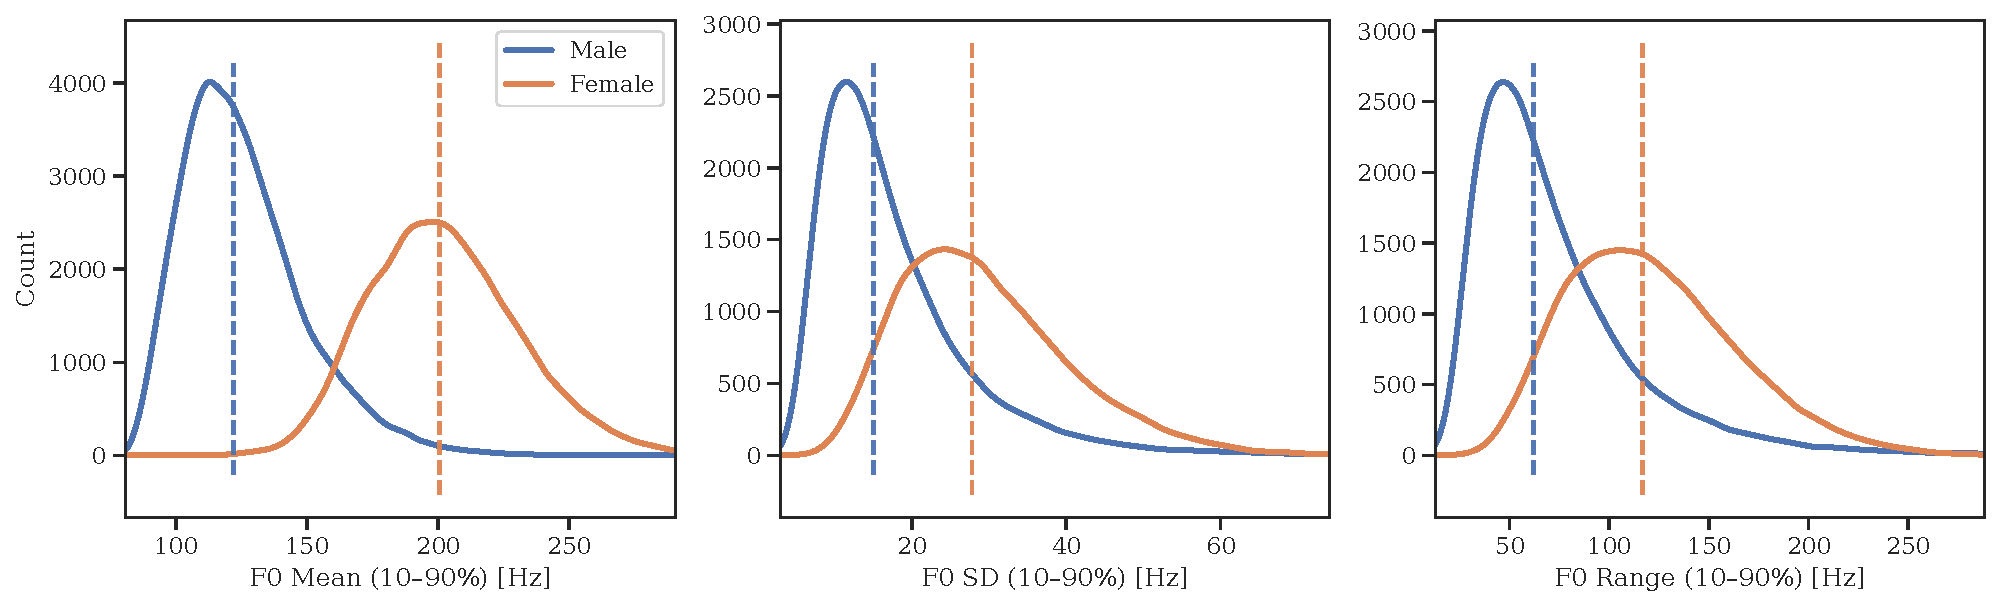
\includegraphics[width=\textwidth]{Fig1_Prosody_Gender.pdf}
  \caption{Prosodic operating regimes (10--90\% trimmed) stratified by gender. Kernel density curves (scaled to counts: $N{=}121{,}813$; Male $=65{,}214$, Female $=56{,}599$) are shown for $F_0$ Mean, SD, and range. Vertical dashed lines mark group medians.}
  \label{fig:prosody_gender}
\end{figure*}

\begin{figure}[t]
  \centering
  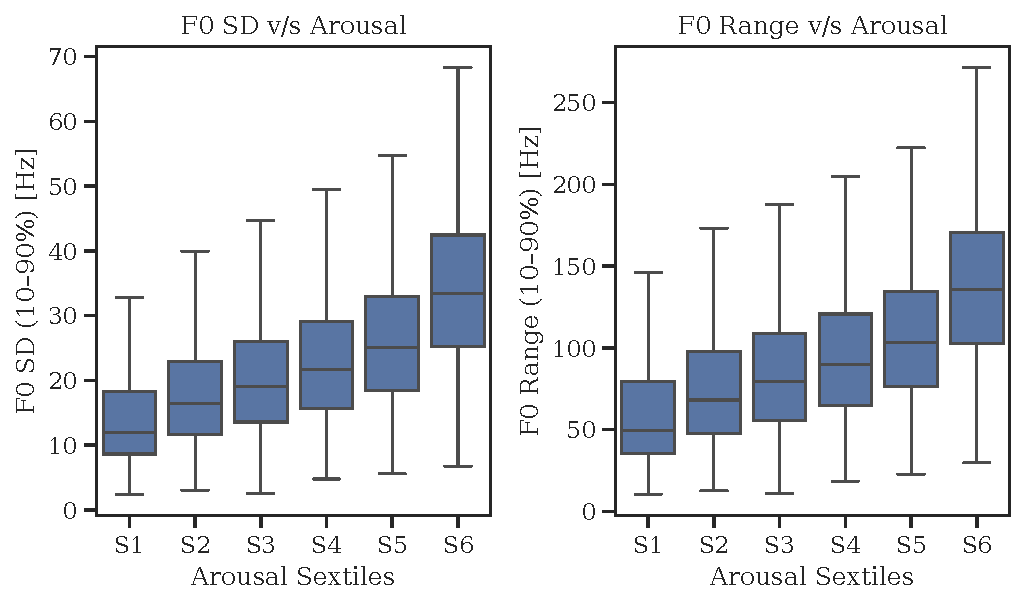
\includegraphics[width=\linewidth]{Fig2_Prosody_Arousal_Bins.pdf}
  \caption{State-driven $F_0$ expressivity across arousal sextiles (S1--S6). Boxplots summarize 10--90\% trimmed $F_0$ standard deviation and $F_0$ range within arousal bins ($N{=}121{,}813$).}
  \label{fig:prosody_arousal}
\end{figure}

\begin{figure}[t]
  \centering
  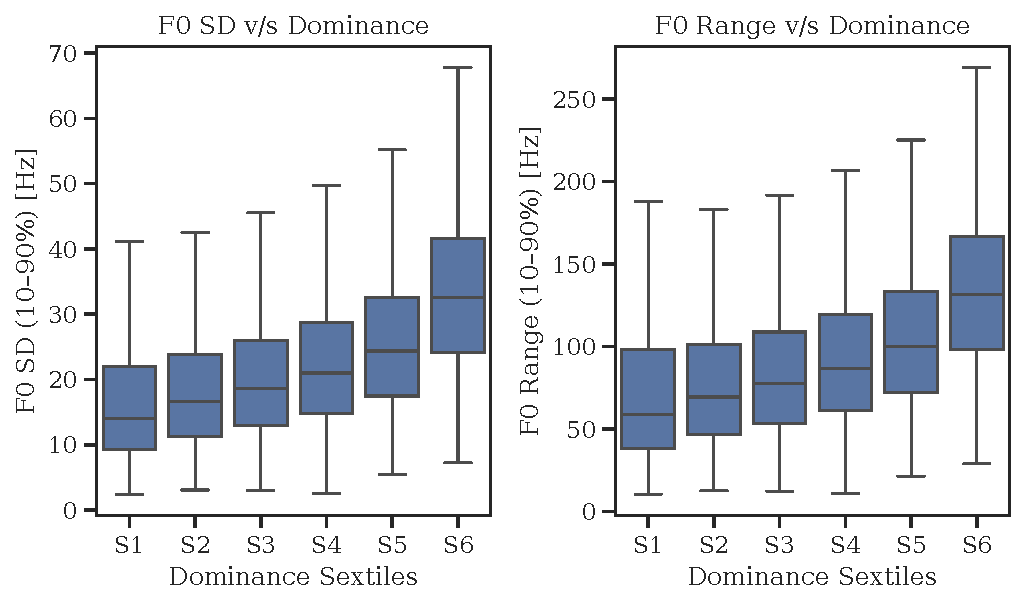
\includegraphics[width=\linewidth]{Fig3_Prosody_Dominance_Bins.pdf}
  \caption{$F_0$ expressivity across dominance sextiles (S1--S6). Boxplots summarize 10--90\% trimmed $F_0$ standard deviation and $F_0$ range within dominance bins ($N{=}121{,}813$).}
  \label{fig:prosody_dominance}
\end{figure}

We summarize the operating regimes of conversational prosody and rhythm and quantify how these regimes vary with speaker and interaction factors.
Throughout, $N$ denotes the number of usable speaker-channel samples satisfying the subset criteria for a given figure/table, and hours denote total speech duration aggregated over those usable samples (reported as interaction-time). 
We use the term ``expressivity'' to jointly refer to the range and standard deviation of $F_0$.
Table~\ref{tab:pooled_regimes_single} reports pooled reference ranges, Table~\ref{tab:gender_effects} summarizes two-group gender effects, and Table~\ref{tab:state_age_effects} summarizes continuous state (arousal, dominance) and age effects. 
Since the corpus is large, we report effect sizes in addition to significance tests: for two-group comparisons we use the Mann--Whitney $U$ test with Cliff's $\delta$ to quantify distributional separation without assuming normality \cite{cliff1993dominance}; for continuous co-variates (arousal, dominance) we use Spearman rank correlation $\rho$ to capture monotonic associations robustly \cite{spearman1961proof}; and for age-bin comparisons we use the Kruskal--Wallis test with $\epsilon^2$ as an effect size for multi-group differences \cite{kruskal1952use, tomczak2014need}. 
When we report pooled regimes, this reflects that additional metadata factors we screened produced negligible effect sizes for the corresponding metric, otherwise, we present stratified reference regimes for the dominant drivers.
We compared Naturalistic and Improvised subsets for the global prosodic and temporal metrics and observed negligible effect sizes, so we pool them for a compact regime characterization.

\subsection{Prosodic Regimes}
We characterize conversational prosody using robust 10--90\% trimmed $F_0$ statistics that summarize $F_0$ mean, SD, and range.
Figure~\ref{fig:prosody_gender} shows that the mean $F_0$ is strongly gender-conditioned, with large distributional separation that makes pooled absolute-$F_0$ targets inappropriate for evaluation. 
This aligns with long-standing evidence that anatomical/physiological differences yield distinct habitual $F_0$ regimes across speakers \cite{traunmuller_acoustic_2000, titze_toward_1994}.

Beyond this baseline conditioning, Figures~\ref{fig:prosody_arousal} and \ref{fig:prosody_dominance} show a consistent scaling of prosodic expressivity with interactional state. 
In particular, $F_0$ SD and $F_0$ range increase monotonically across arousal and dominance sextiles obtained with VoxProfile. 
This matches prior work showing that natural speech tends to use a wider $F_0$ bandwidth in higher-activation emotional or interactional states, with larger pitch excursions when speakers are more activated or more socially assertive \cite{banziger_role_2005, banse1996acoustic, geng2020acoustic}. 
If the $F_0$ produced by a speaker or an S2S dialogue system stays in a narrow-band variation in high-arousal or high-dominance contexts, it may sound constrained or unnatural even when the mean $F_0$ is within a typical range \cite{liu2021multiple}.
Prosodic evaluation should therefore include expressivity-sensitive checks in addition to $F_0$ level, and interpret deviations relative to reference distributions stratified by arousal and dominance \cite{pell_emotional_2011, xu_speech_2005}.

\subsection{Temporal Regimes}

\begin{figure*}[t]
  \centering
  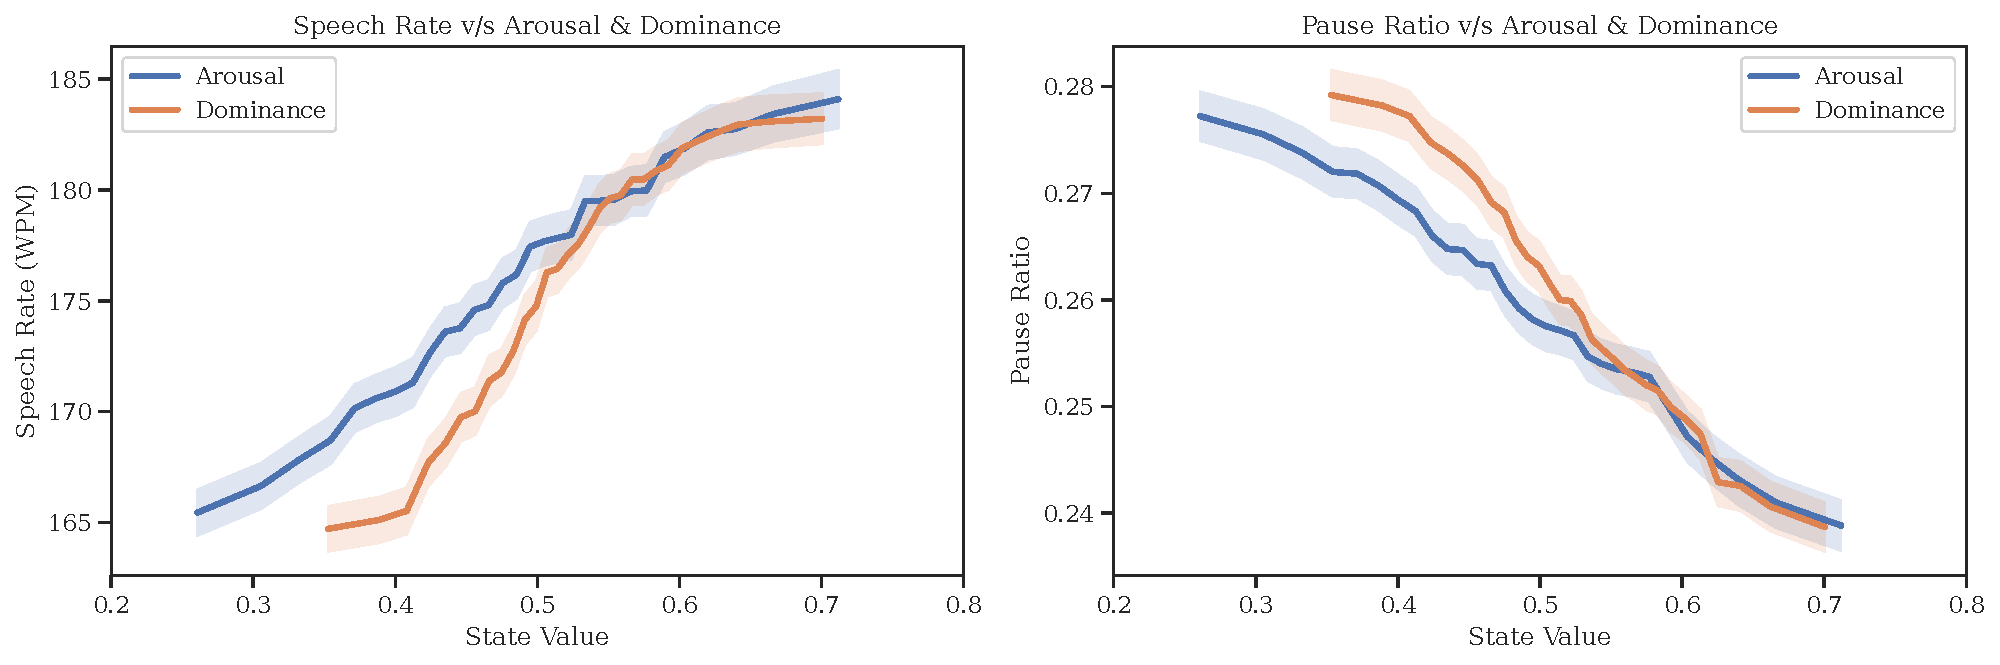
\includegraphics[width=\textwidth]{Fig4_Temporal_Trends_State.pdf}
  \caption{Conversational rhythm varies with interactional state. Smoothed trends show speech rate (left) and pause ratio (right) as functions of arousal and dominance (0--1). Trends are computed from equal-count bins ($N{=}91{,}471$) over the state axis, followed by smoothing. Shaded bands indicate $\approx95\%$ uncertainty (SEM-based). Bins with sparse data are omitted to reduce unstable end effects.}
  \label{fig:temporal_state}
\end{figure*}

\begin{figure*}[t]
  \centering
  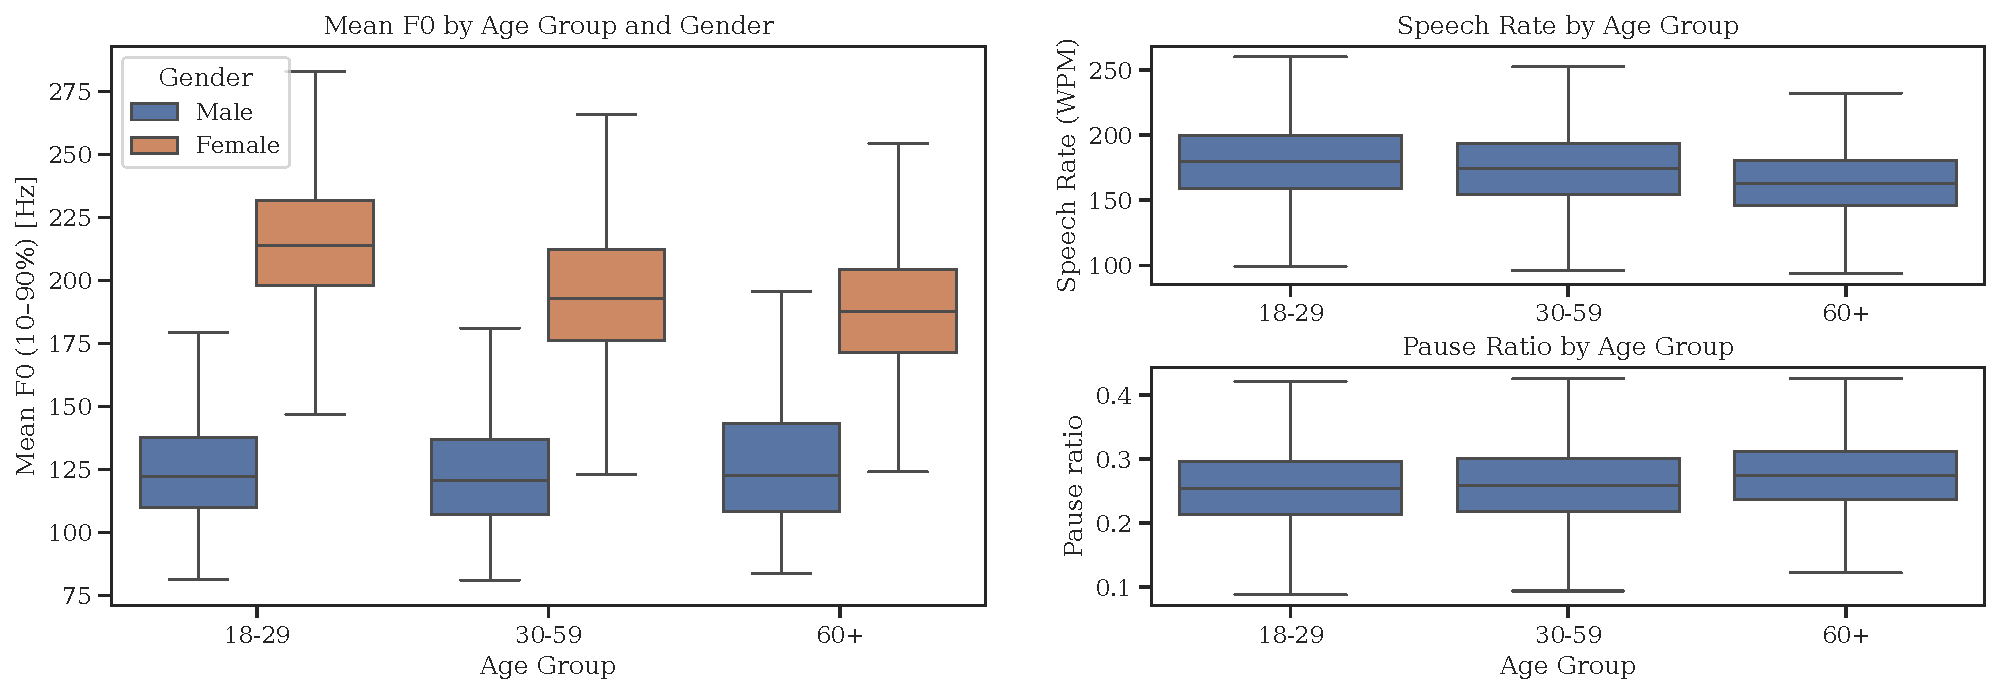
\includegraphics[width=\textwidth]{Fig5_Age_Prosody_Temporal.pdf}
  \caption{Age-group effects on prosody and rhythm. Left: mean $F_0$ (10--90\% trimmed) across Vox-Profile age bins (18--29 / 30--59 / 60+) stratified by gender ($N{=}118{,}033$). Right: speech rate and pause ratio distributions across the same age bins ($N{=}88{,}287$).}
  \label{fig:age_effects}
\end{figure*}

We characterize conversational rhythm with speech rate and pause ratio, capturing how time is allocated between verbal output and silence.
Figure~\ref{fig:temporal_state} shows state dependence, where speech rate increases with arousal and dominance, while pause ratio decreases. 
This coupled pattern is consistent with classic observations that perceived ``speed of talking'' is driven heavily by the structure and frequency of pauses rather than articulation speed alone, motivating joint descriptions of conversational rhythm \cite{goldman1958speech, goldman1961significance}.
It also agrees with applied-linguistics evidence that conversational speech rates occupy a bounded range while varying by situation and interaction \cite{tauroza_speech_1990, nishizawa2024authenticity}.

Age further shifts temporal regimes in a way that matters operationally for evaluation. 
% The "trap" here, that we cannot solve (so you need to leave it as it is) is that you really don't have age annotation in this dataset and these conclusions just describe the way the VoxProfile models are behaving, not necessarily humans. Although if we assume that VoxProfile was well trained, the ideas will be valid. We might want to add a comment like this at the end of the paper, somewhere, if we have space.
Figure~\ref{fig:age_effects} shows that age bins are associated with changes in speech rate and pause ratio, implying that ``natural'' timing targets are not universal across age. 
This result complements prior conversation analyses showing that timing patterns can index participation style and interactional dynamics \cite{campbell2008individual}. 
For conversational systems, the practical implication is that timing-based diagnostics should evaluate pace and pausing jointly, and condition on age (when available).  

\section{Implications for Speech Technology}\label{sec:implications}

\subsection{Human operating regions}\label{sec:operating_regions}
The distributions in Section~\ref{sec:regimes} provide operating regions for conversational prosody and rhythm. 
As a practical diagnostic, large deviations from these regions can flag outputs that are unlikely under human conversational behavior, particularly when systems must produce state-appropriate $F_0$-expressivity and timing. 
Since our results show strong conditioning effects, meaningful comparisons should use matched reference strata rather than a single pooled baseline.

\subsection{Toward evaluation frameworks}\label{sec:toward_frameworks}
These findings motivate evaluation frameworks grounded in empirical conversational behavior. 
% Reference regimes can serve as calibrated targets for generation and as interpretable diagnostics for analysis, helping identify whether unnaturalness stems from compressed prosodic expressivity, mismatched pacing, or atypical pause allocation. 
% A natural next step is to extend the cue set and learn an aggregate assessment model that maps speech to a scalar conversational-naturalness score while retaining per-cue interpretability for debugging and iteration.
Reference regimes can be used as a lightweight alignment check for S2S agents: given an output waveform, compute the same metrics, select the appropriate reference stratum (like sex label or predicted state), and report percentile deviations or out-of-range flags per metric. 
This provides actionable diagnostics during development (which dimension is off and in what direction) and can be aggregated into a simple multi-cue score while preserving per-metric interpretability for debugging.

\subsection{Limitations}\label{sec:limitations}
This study is descriptive. 
It provides large-scale reference distributions and conditioning effects, but does not yet map deviations to perceptual thresholds or user-rated interaction quality. 
Results are derived from a single English dyadic corpus. 
Operating regions may shift with language, domain, recording conditions, and interaction setting. 
Predicted age/arousal/dominance are derived from Vox-Profile models rather than self-reports, so observed stratification effects should be interpreted as model-conditioned annotations and validated against ground-truth metadata where available.
The analysis uses a binary sex label predicted from voice and hence does not model non-binary gender identities.
Future work should validate these regimes against human judgments and system outputs across multiple datasets and languages.

\section*{Acknowledgment}

The preferred spelling of the word ``acknowledgment'' in America is without 
an ``e'' after the ``g''. Avoid the stilted expression ``one of us (R. B. 
G.) thanks $\ldots$''. Instead, try ``R. B. G. thanks$\ldots$''. Put sponsor 
acknowledgments in the unnumbered footnote on the first page.

\section*{References}

Please number citations consecutively within brackets \cite{b1}. The 
sentence punctuation follows the bracket \cite{b2}. Refer simply to the reference 
number, as in \cite{b3}---do not use ``Ref. \cite{b3}'' or ``reference \cite{b3}'' except at 
the beginning of a sentence: ``Reference \cite{b3} was the first $\ldots$''

Number footnotes separately in superscripts. Place the actual footnote at 
the bottom of the column in which it was cited. Do not put footnotes in the 
abstract or reference list. Use letters for table footnotes.

Unless there are six authors or more give all authors' names; do not use 
``et al.''. Papers that have not been published, even if they have been 
submitted for publication, should be cited as ``unpublished'' \cite{b4}. Papers 
that have been accepted for publication should be cited as ``in press'' \cite{b5}. 
Capitalize only the first word in a paper title, except for proper nouns and 
element symbols.

For papers published in translation journals, please give the English 
citation first, followed by the original foreign-language citation \cite{b6}.

\bibliographystyle{IEEEtran}
\bibliography{newbib}

\vspace{12pt}
\color{red}
IEEE conference templates contain guidance text for composing and formatting conference papers. Please ensure that all template text is removed from your conference paper prior to submission to the conference. Failure to remove the template text from your paper may result in your paper not being published.

\end{document}
